% ============================================================
\section{Numerical Experiments}
\label{sec:experiments}
We evaluate the proposed simulation-in-the-loop NAMO planner (SiLS)
in cluttered environments with both movable and immovable obstacles.
All components (W-CCG presearch, frontier extraction, and ModeTable prior)
are integrated as described in Sec.~\ref{sec:solution}.
The implementation is in \texttt{Python~3} and simulations are run in
\texttt{PyBullet}~\cite{coumans2019} on a laptop with an Intel
Core i7\textendash1280P CPU. Videos and logs are provided in the
supplementary material.
\begin{figure}
  \centering
  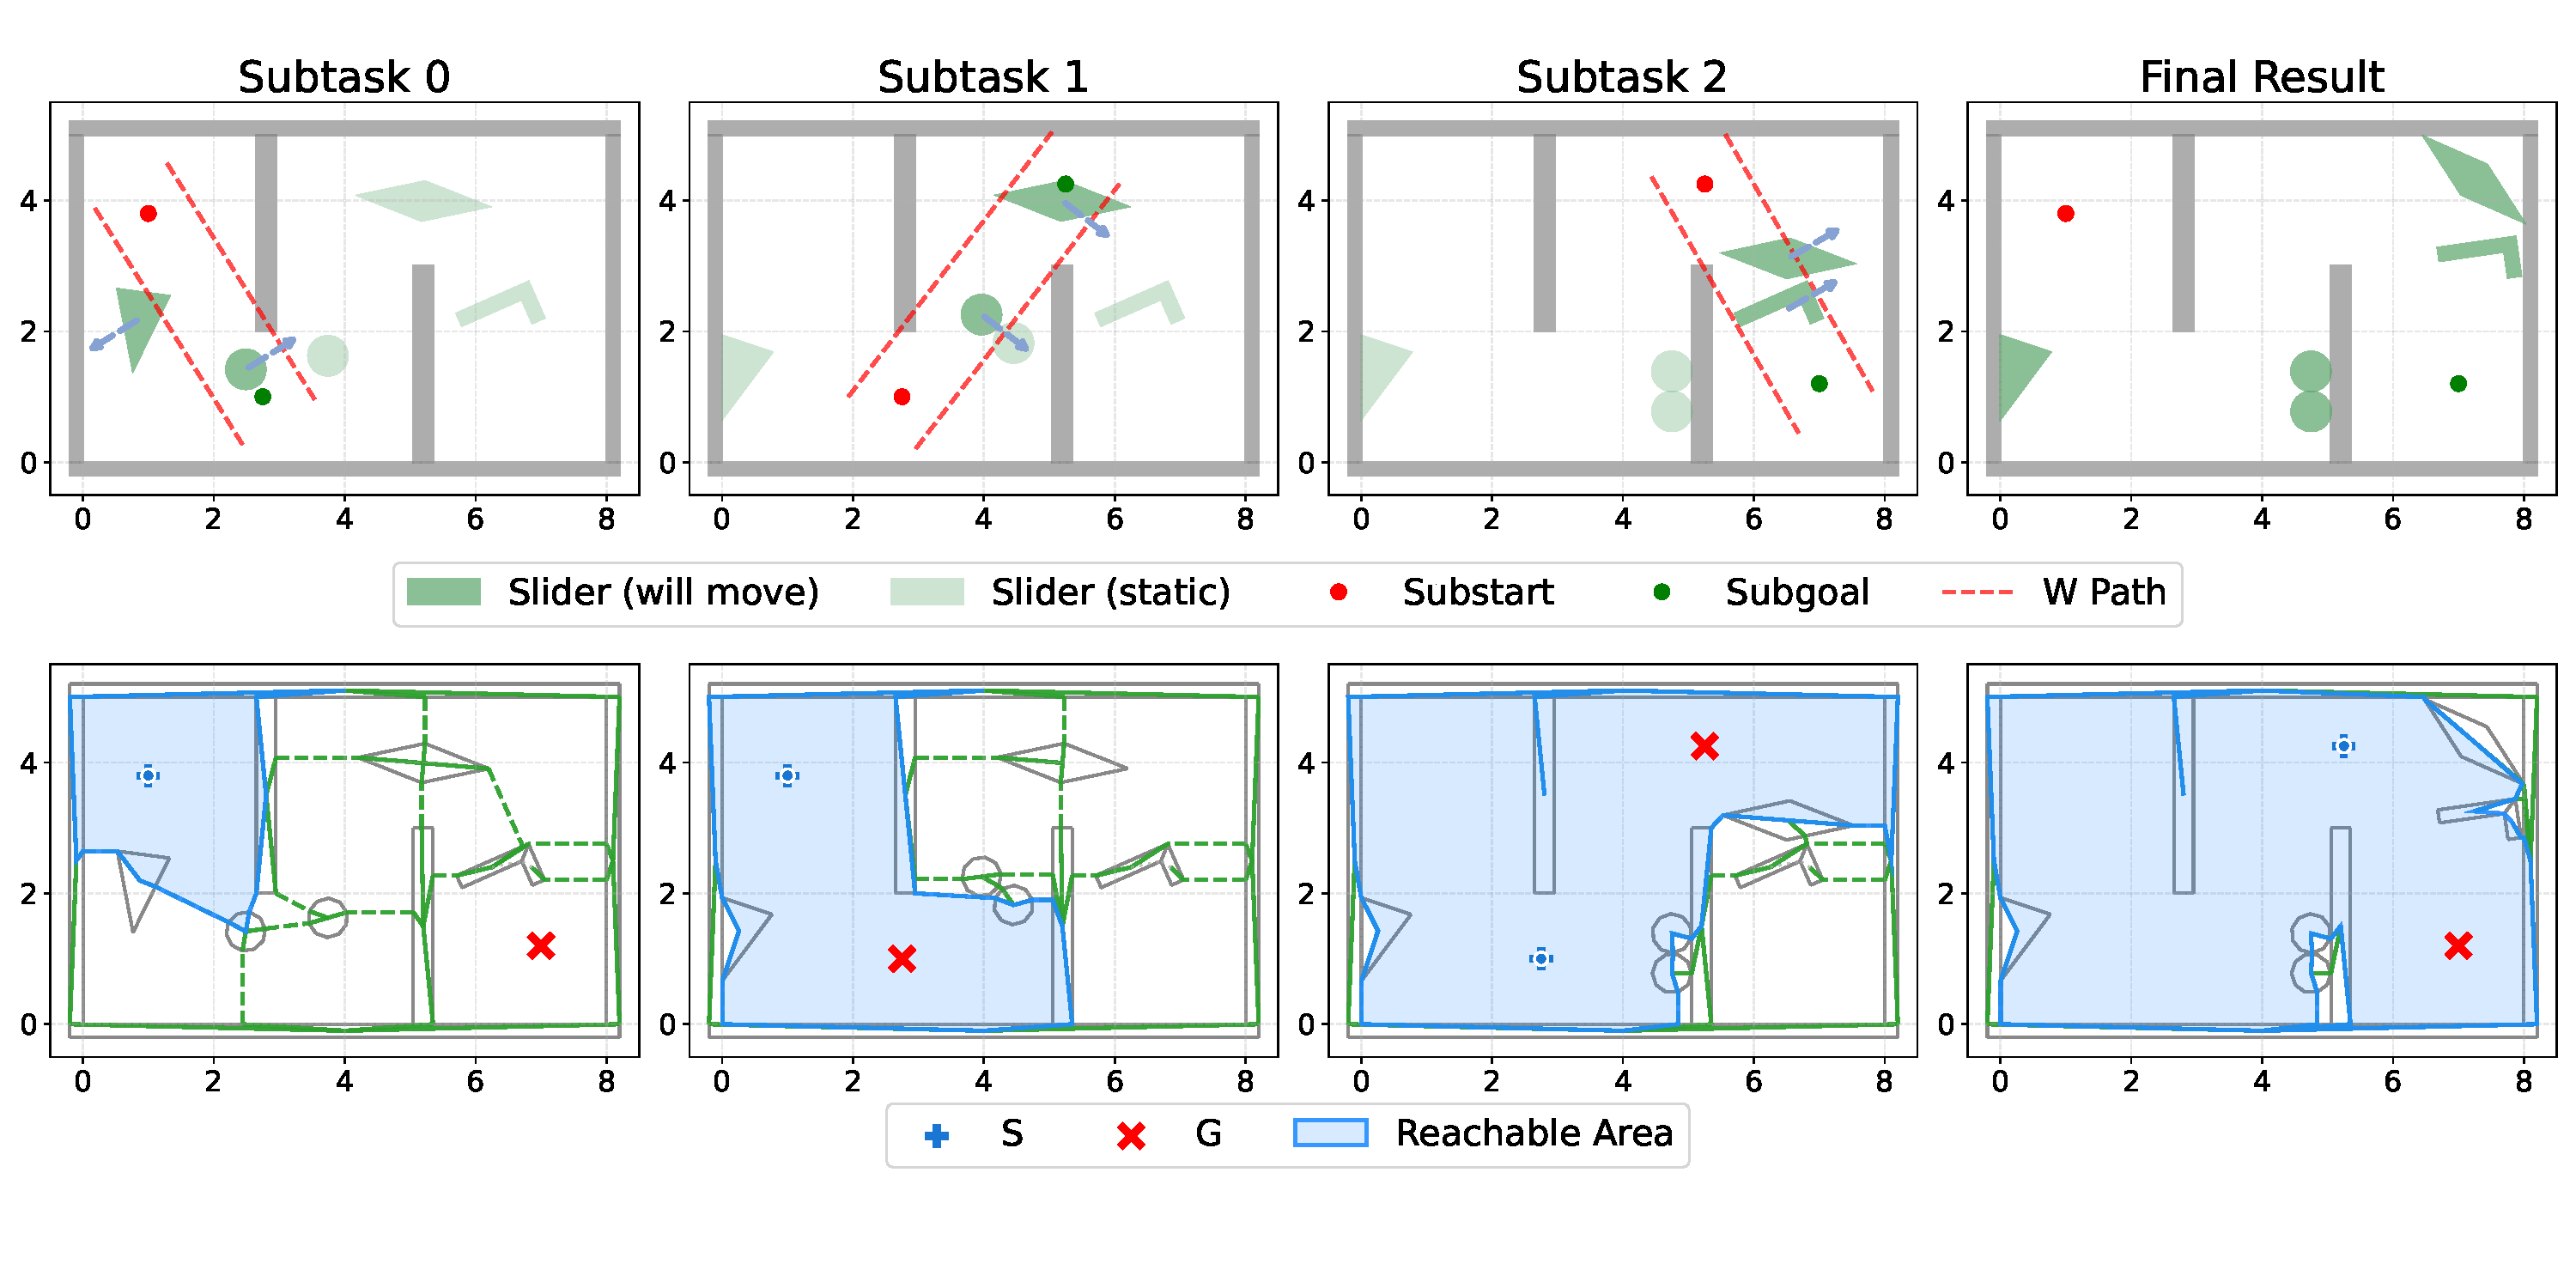
\includegraphics[width=\columnwidth]{figures/SL_Push.pdf}
  \vspace{-10mm}
\caption{SL-Push. Compute(offline) or simulate(sim-in-the-loop) the pushing directions for movable obstacles along the W-width straight path from sub-start to sub-goal. Top: Pushing steps. Bottom: Reachable region changes during pushing}
\end{figure}

\begin{figure}
  \centering
  \vspace{-3mm}
  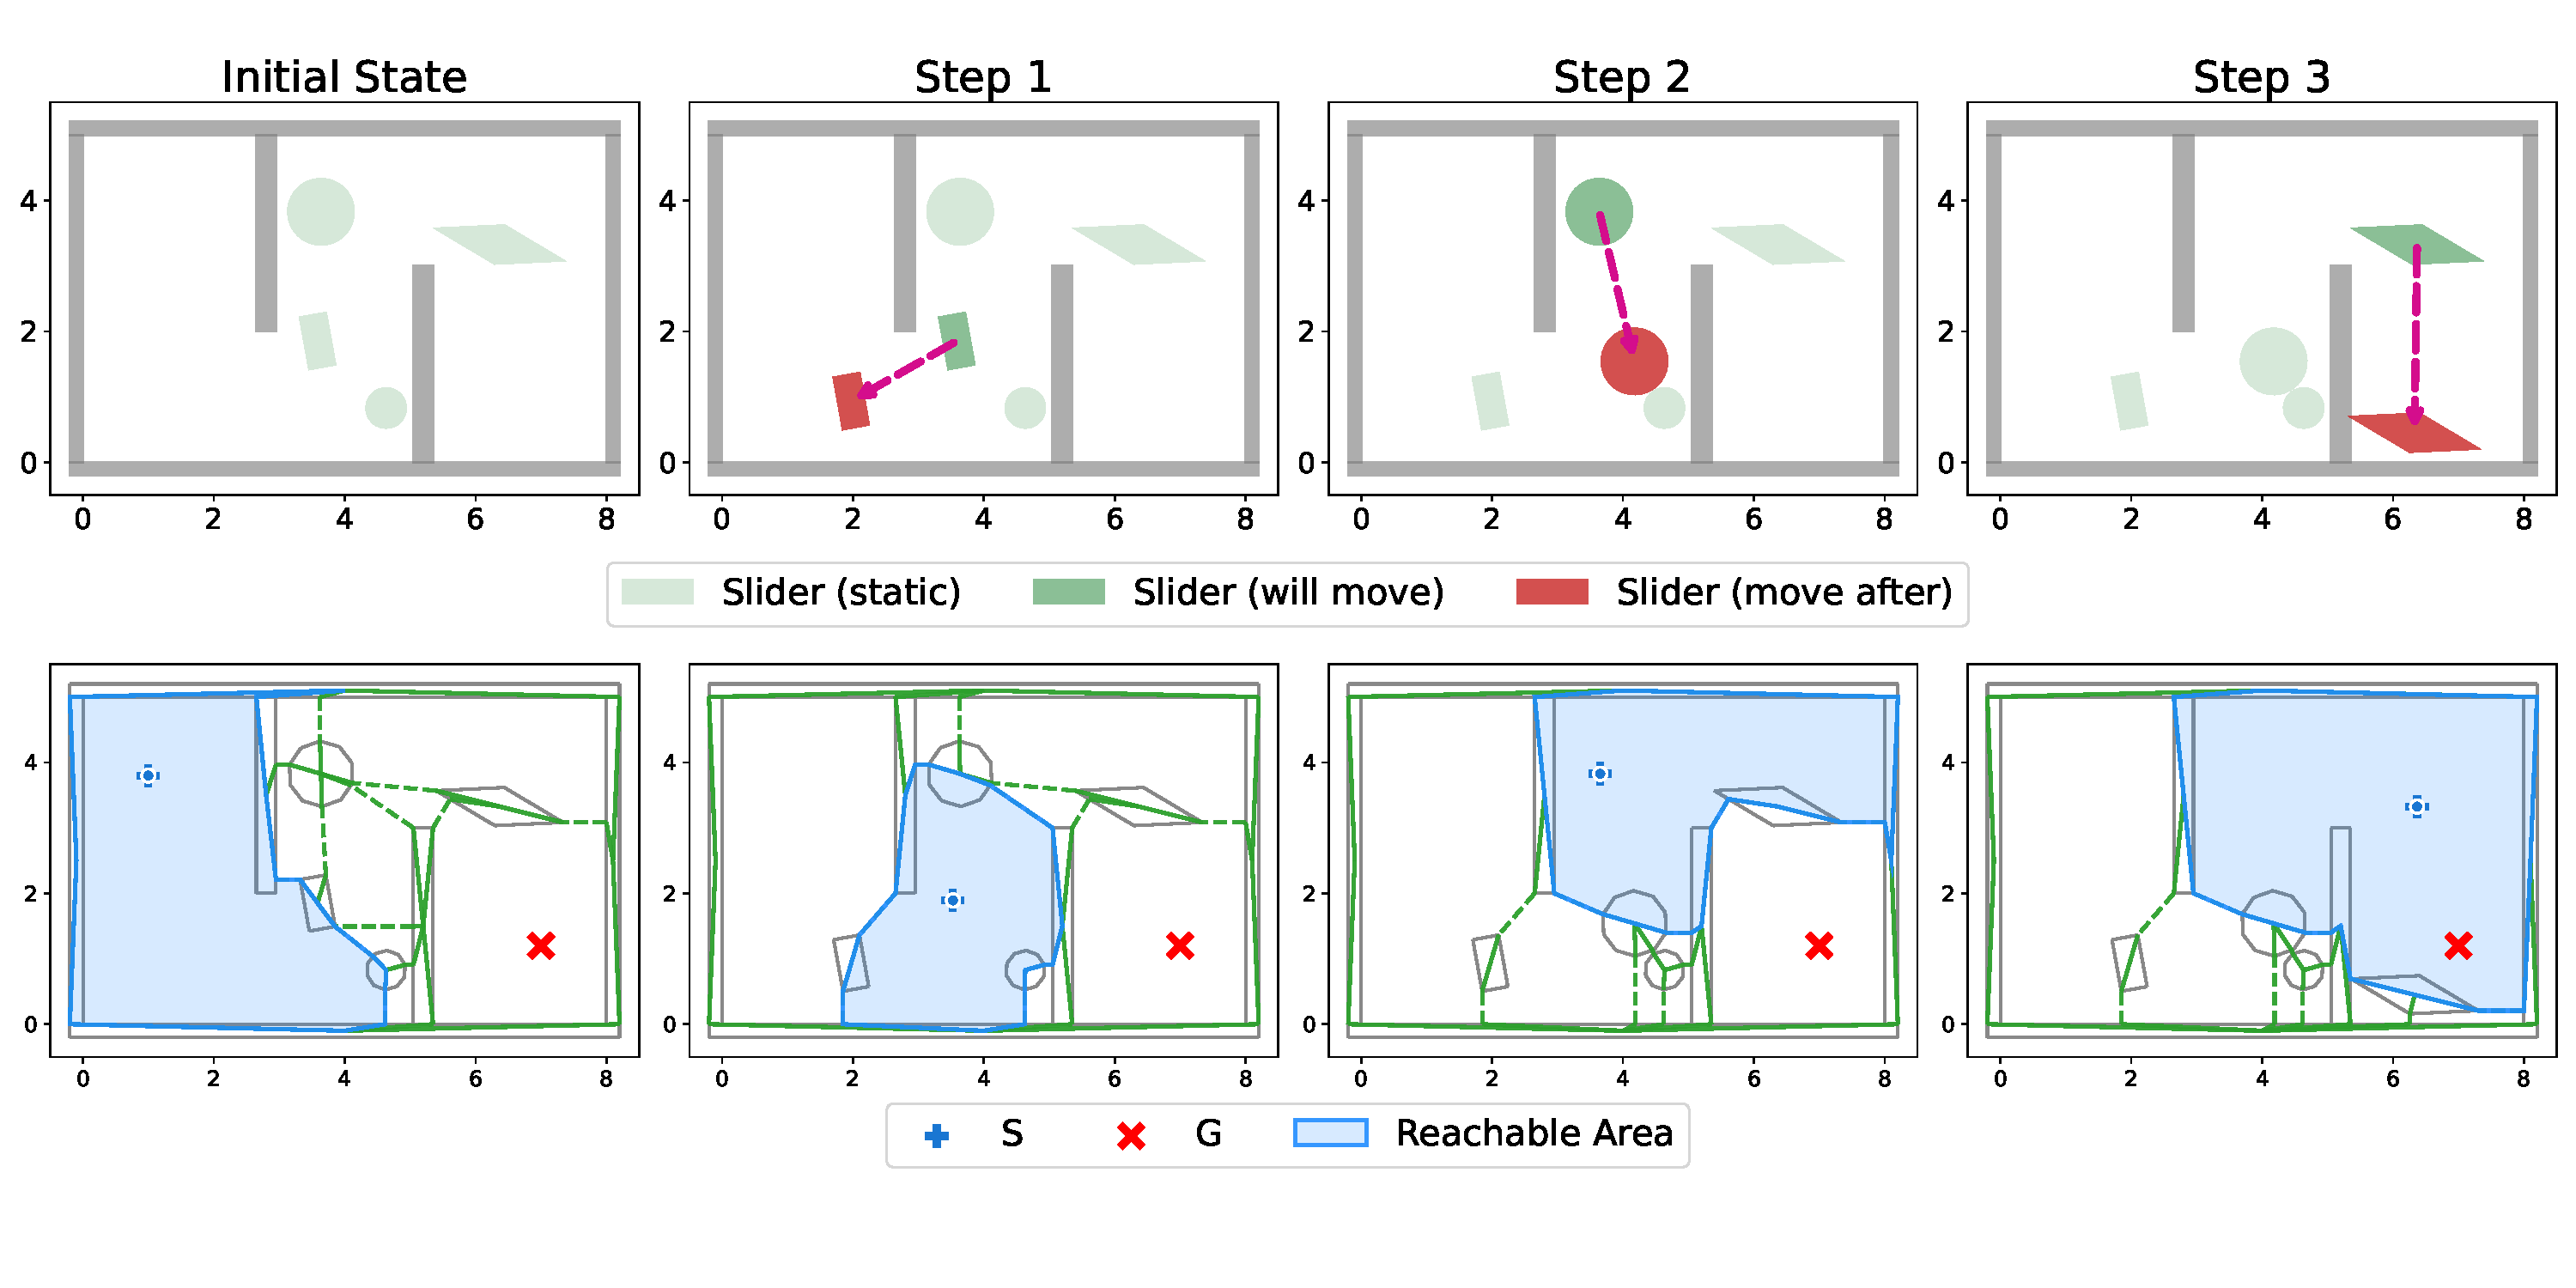
\includegraphics[width=\columnwidth]{figures/Rec_NAMO.pdf}
  \vspace{-10mm}
\caption{Rec-NAMO. Rec-NAMO builds path segments sequentially but fails to construct the full width-w path from start to goal. Top: Pushing steps. Bottom: Reachable region changes during pushing}
\end{figure}



% ========================================
\subsection{Numerical Simulations}
\label{subsec:sim}
% ========================================
\begin{figure}
  
\end{figure}
\subsubsection{\change{Setup}}
\label{subsec:sim-setup}
\change{
The physics step is $\Delta t = 1/120$\,s and the control period is
$1/40$\,s. Robots are disk/box pushers with risk radii consistent with
the $W$-clearance definition. Movable obstacles have masses uniformly
sampled in $[5,15]$\,kg; immovables are modeled with mass $0$.
A trial succeeds when a $W$-clear path from start to goal exists and the
target reaches its goal disc.
}

\textbf{Workspace and scenarios.}
We use a \emph{nominal scenario} with an $8{\times}5$\,m bounded
workspace, two internal bars (bottlenecks), and a mixed pool of movable
shapes (curved and polygonal, including rings, ellipses, X/T/L/diamond,
arrow-like, rectangles, and cylinders). Two robots start in the lower
left; the target goal lies on the right side. Movables are randomly
placed with a minimum separation. We test \(10\text{--}15\) objects
over multiple seeds.

\textbf{Geometry and caching.}
Collision checks use polygon/curve-edge models with convex
decomposition when needed. Ray--edge queries for frontiers are
vectorized with AABB culling. Frontier loops are cached by signatures and
transitions $(\mathcal{L},g)\!\mapsto\!\mathcal{L}'$ are memoized.

\subsubsection{\change{Algorithm Configuration}}
\label{subsec:algo-config}
\change{
Unless stated otherwise: per-task simulation horizon $=80$ steps,
up to $64$ candidate push tasks per expansion, and priority
$f = g + \widehat{\mathsf{Cost}}_{\text{to-go}}$ with heuristic factor $10$.
Gap sampling uses a softmax with temperature $0.05$.
ModeTable is enabled (auto-baked if missing).
A \emph{quick-pass} geometry screen may skip physics if a reference
rollout already clears the gap; otherwise a short-horizon simulation with
early stop is used. To avoid premature termination, a
\emph{deferred-reinsertion} rule keeps high-value but temporarily
unexpanded nodes in the queue and revisits them later.
}

\subsubsection{\change{Baselines}}
\label{subsec:baselines}
We compare against three representative families, all using the same
$W$-clearance criterion and contact models:

\textbf{DFS-WCCG:} Simulation-in-the-loop depth-first search 
that shares our physics predictor and $W$–CCG for goal checking.
Each node is a snapshot; actions are four fixed axis-aligned pushes 
${!\leftarrow,\rightarrow,\uparrow,\downarrow!}$ 
applied to any movable object (branching $\le 4n$ for $n$ objects).

\textbf{SL-Push:} Straight-line (or waypointed) route; blockers are
cleared by (i) off-line minimal normal displacements or
(ii) sim-in-the-loop normal pushes from near to far.

\textbf{Rec-NAMO:} Recursive routing/pushing on a cost-weighted
  visibility graph: Dijkstra for routing, push-decomposition for local
  clearing; failures prune edges and replan.


\subsubsection{\change{Metrics}}
\label{subsec:metrics}
We report success rate, wall-clock time, number of node expansions,
number of simulated pushes, cumulative push time, average presearch
cost-to-go, quick-pass ratio, early-stop ratio, and worker-pool
utilization. Results are averaged over 10 seeds unless noted.

% ==============================
\subsubsection{Main Results}
\label{subsec:main-results}
Table~\ref{tab:main} summarizes performance on the nominal scenario.
SiLS attains higher success with fewer simulations and lower time due to:
(i) frontier-based gap ranking, (ii) ModeTable-guided push directions,
and (iii) quick-pass/early-stop. Deferred reinsertion prevents
priority-queue starvation by revisiting previously generated high-value
nodes when a batch of actions fails.

\begin{table}[t]
  \centering
  \begin{threeparttable}
  \caption{Performance on the nominal scenario with push-count (mean $\pm$ std).}
  \label{tab:main-push}
  \vspace{2pt}
  
  % 🔑 在这里调节列间距
  \setlength{\tabcolsep}{2.3pt} % 默认是 6pt,调小
  
  \begin{tabular}{lccccc}
  \toprule
  Method & Succ.~(\%) & \#PT (s) & \#ET (s) & \#Sims & \#Pushes \\
  \midrule
  DFS-WCCG            & 25 & timeout & N/A & - & - \\
  SL-Push (off-line)  & 62.5 & 0.02 & 145.147 & 0 & 7 \\
  SL-Push (sim)       & 75 & 25.09 & 246.825 & 16 & 8 \\
  Rec-NAMO            & 37.5 & 10.45 & 179.262 & 0 & 7 \\
  \textbf{SiLS (ours)}& \textbf{--} & \textbf{--} & \textbf{--} & \textbf{--} & \textbf{--} \\
  \bottomrule
  \end{tabular}
  
  \begin{tablenotes}[flushleft]\footnotesize
  \item \textbf{Metrics.} \emph{Succ.} = success rate; \emph{\#PT} = planning time; \emph{\#ET} = execution time;
  \emph{\#Sims} = simulations invoked; \emph{\#Pushes} = length of executed push sequence.
  \end{tablenotes}
  \end{threeparttable}
  \end{table}
  


\subsubsection{Ablations}
\label{subsec:ablations}
We remove one component at a time: (i) W-CCG presearch (random gap order),
(ii) ModeTable prior (fallback “away\,+\,jitter” only),
(iii) quick-pass/early-stop (always full physics),
(iv) deferred reinsertion (terminate on empty queue).
Table~\ref{tab:ablation} shows consistent drops in success and increased
time/\#Sims when any component is disabled.

\begin{table}[t]
  \centering
  \caption{Ablations on the nominal scenario (fill with measurements).}
  \label{tab:ablation}
  \vspace{2pt}
  
  % 🔑 调整列间距和行距(只对本表生效)
  {%
  \setlength{\tabcolsep}{3pt} % 列间距缩小
  \renewcommand{\arraystretch}{0.9} % 行距缩小
  
  \begin{tabular}{lcccc}
  \toprule
  Variant & Succ.~(\%) & Time (s) & \#Sims & Quick-pass (\%) \\
  \midrule
  SiLS (full)            & -- & -- & -- & -- \\
  \ \ w/o presearch      & -- & -- & -- & -- \\
  \ \ w/o ModeTable      & -- & -- & -- & -- \\
  \ \ w/o quick-pass/ES  & -- & -- & -- & -- \\
  \ \ w/o reinsertion    & -- & -- & -- & -- \\
  \bottomrule
  \end{tabular}
  }% 局部作用域结束
  
  \end{table}
  

\subsubsection{Efficiency and Scalability}
\label{subsec:eff}
\textbf{Frontier caching} makes BugPlanner near-linear in visible edges.
\textbf{Parallel prediction} uses a persistent worker pool with per-round
broadcast of snapshots and reachable-contact sets to reduce IPC.
\textbf{Quick-pass} and \textbf{early-stop} skip or truncate physics when
geometry suffices. \textbf{Deferred reinsertion} maintains steady depth
growth even when many pushes are rejected.

\subsubsection{Qualitative Results}
\label{subsec:qual}
Figure~\ref{fig:qual} shows a typical run: frontiers and ranked gaps,
a top-ranked gap sequence, simulated pushes that widen bottlenecks, and
the final $W$-clearance path. Per-step overlays and GIFs are produced by
a lightweight snapshot logger.

% \begin{figure}[t]
% \centering
% \includegraphics[width=0.98\linewidth]{figures/qual_demo.pdf}
% \caption{Representative run: frontier (blue), ranked gaps (color-coded by
% predicted cost), simulated pushes (red), and the resulting
% $W$-clearance path (green).}
% \label{fig:qual}
% \end{figure}

\subsubsection{Reproducibility}
\label{subsec:repro}
Random seeds are fixed, JSONL snapshots are logged, and the driver and
scenario generator are released. ModeTable entries are auto-generated if
absent to ensure repeatability across machines.

